\newpage
\chapter{Netsimile}
\section{Eindimensionales Signal}
\begin{figure}
	\centering
	\subfloat[Caption for sub-figure1]{
		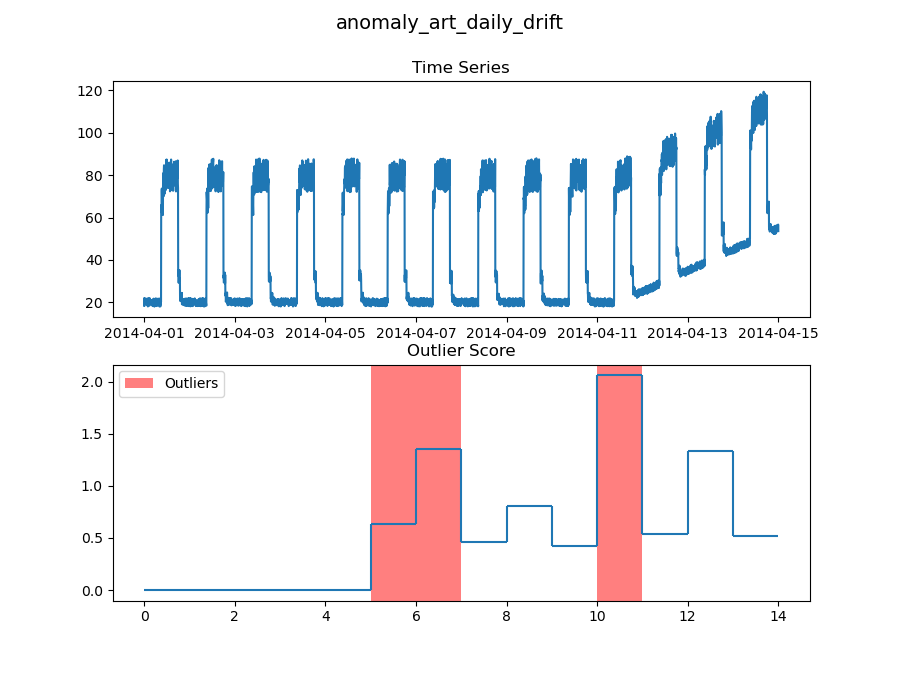
\includegraphics[width=0.5\textwidth]{fig/resultsNetismile/1D/anomaly_art_daily_drift}}
	\subfloat[Caption for sub-figure1]{
		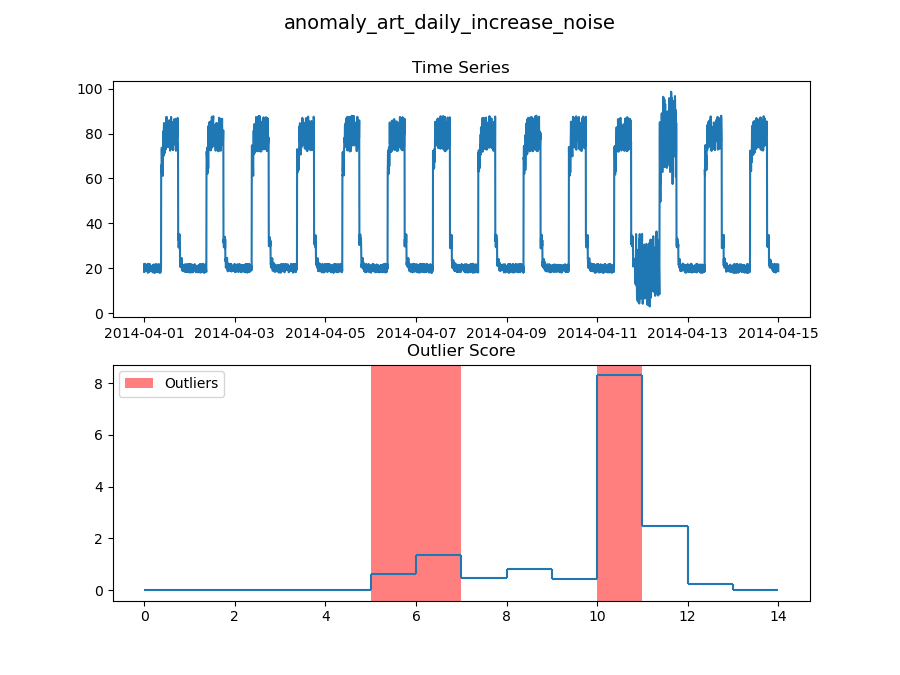
\includegraphics[width=0.5\textwidth]{fig/resultsNetismile/1D/anomaly_art_daily_increase_noise}}
	\qquad
	\subfloat[Caption for sub-figure1]{
		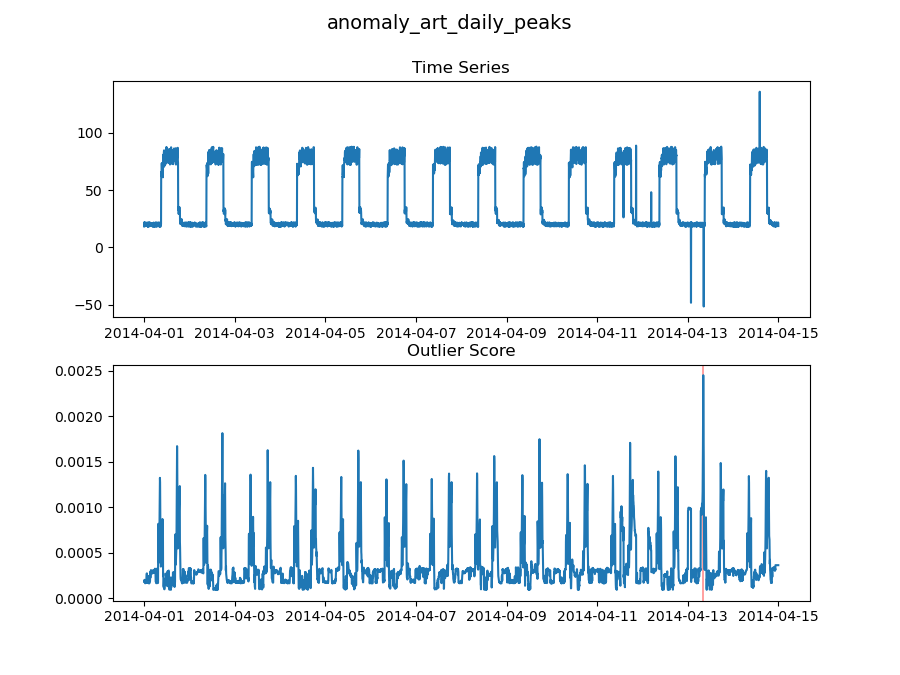
\includegraphics[width=0.5\textwidth]{fig/resultsIsoMap/anomaly_art_daily_peaks}}
	\subfloat[Caption for sub-figure1]{
		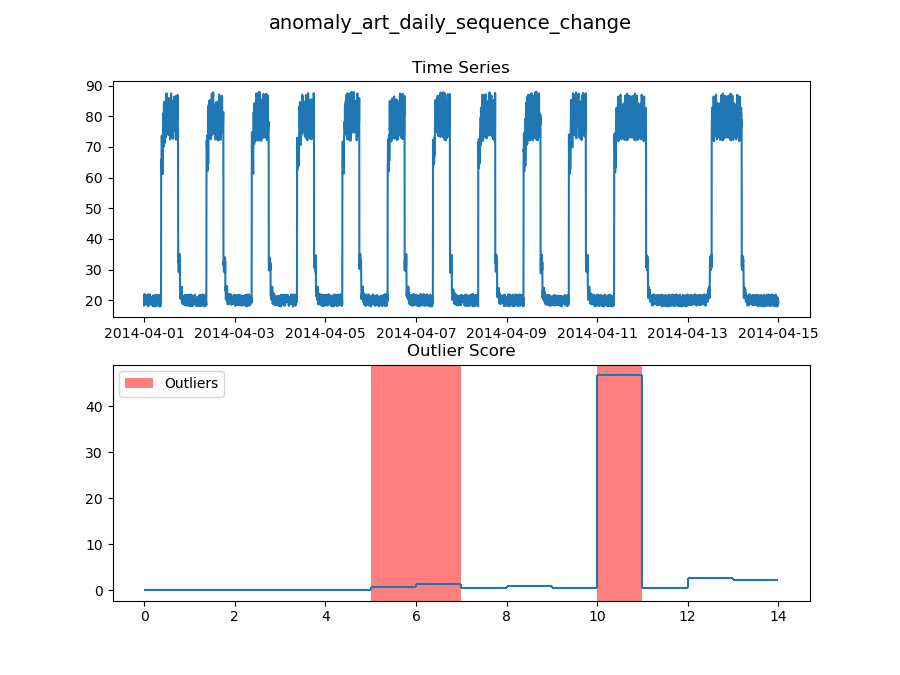
\includegraphics[width=0.5\textwidth]{fig/resultsNetismile/1D/anomaly_art_daily_sequece_change}}
	\qquad
	\label{img:isomappictures1}
\end{figure}
\begin{figure}\ContinuedFloat
	\subfloat[Caption for sub-figure1]{
		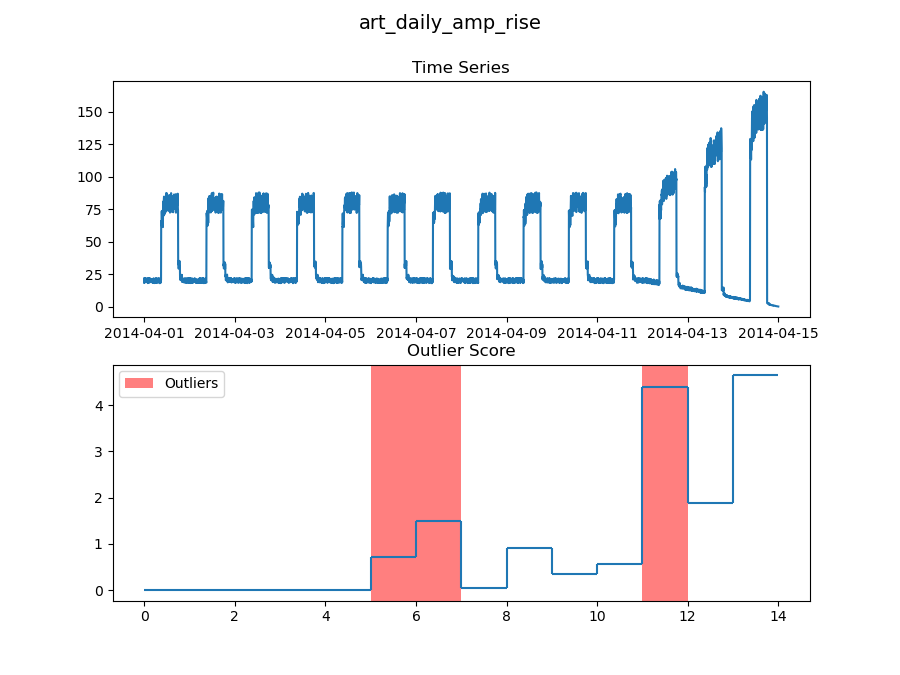
\includegraphics[width=0.5\textwidth]{fig/resultsNetismile/1D/art_daily_amp_rise}}
	\subfloat[Caption for sub-figure1]{
		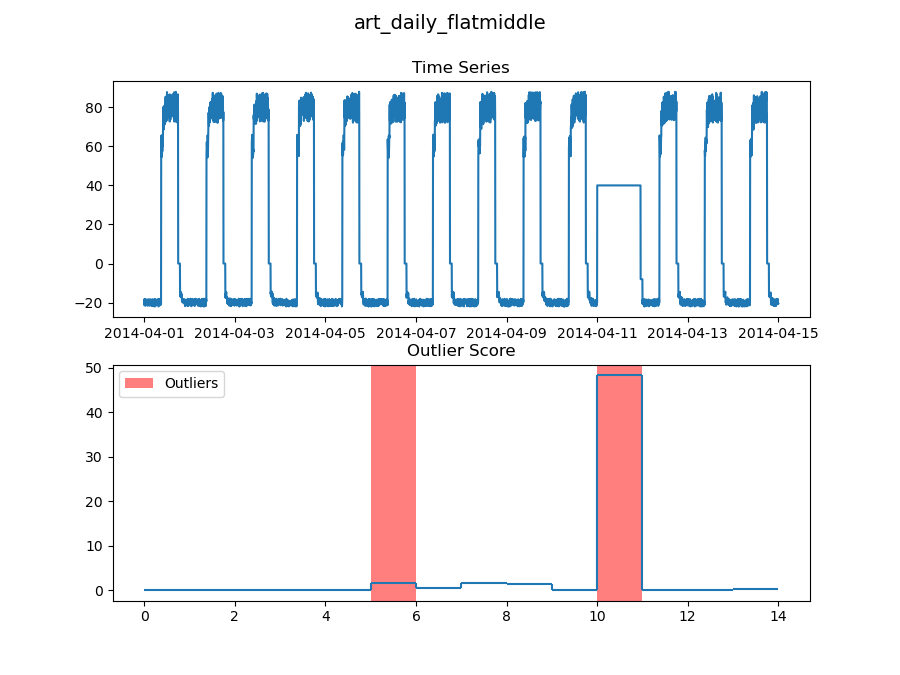
\includegraphics[width=0.5\textwidth]{fig/resultsNetismile/1D/art_daily_flatmiddle}}
	\qquad
	\subfloat[Caption for sub-figure1]{
		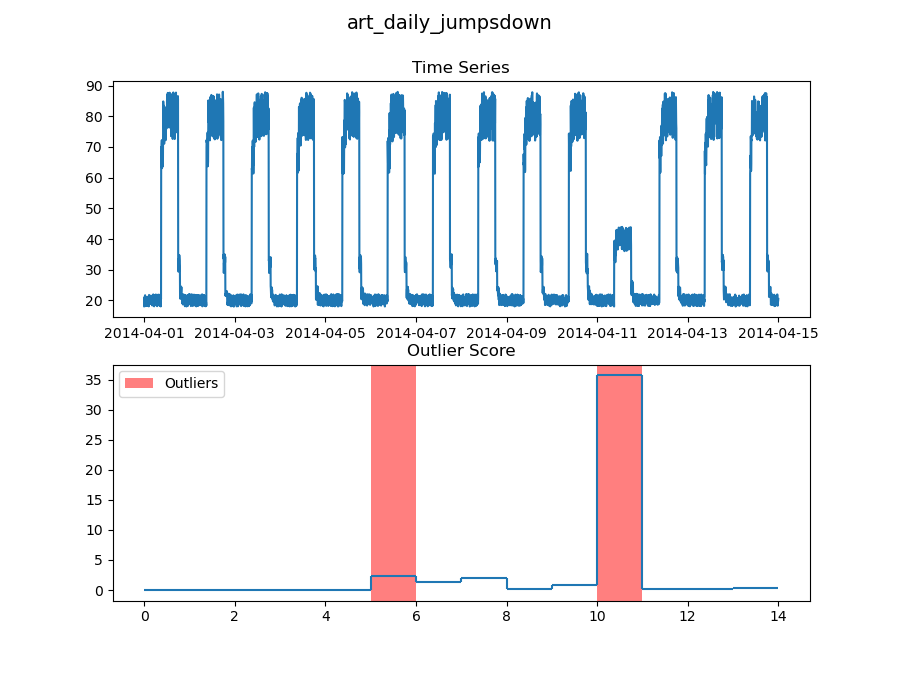
\includegraphics[width=0.5\textwidth]{fig/resultsNetismile/1D/art_daily_jumpsdown}}
	\subfloat[Caption for sub-figure1]{
		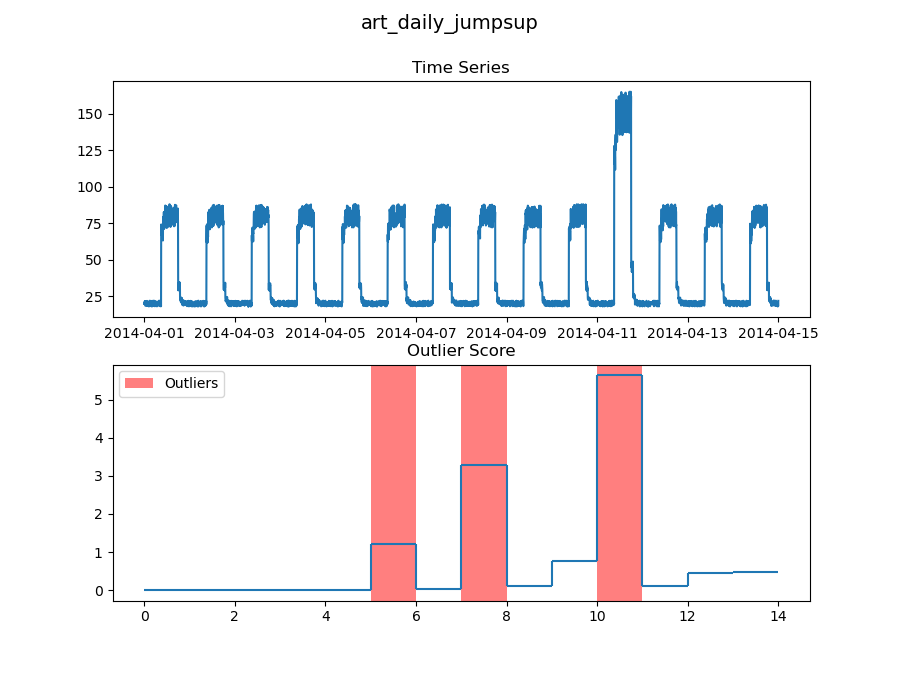
\includegraphics[width=0.5\textwidth]{fig/resultsNetismile/1D/art_daily_jumpsup}}
	\qquad
	\subfloat[Caption for sub-figure1]{
		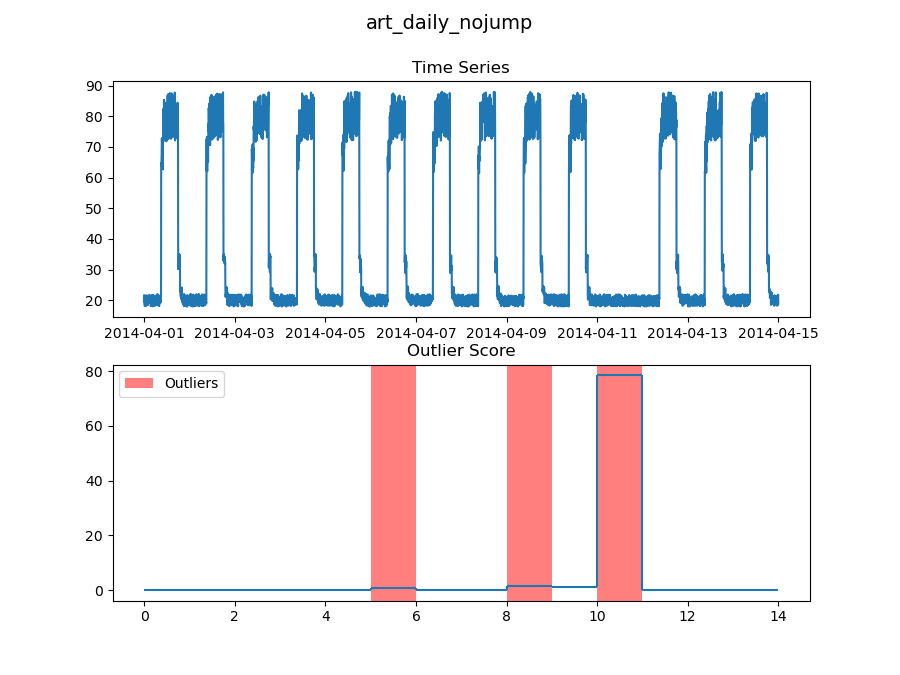
\includegraphics[width=0.5\textwidth]{fig/resultsNetismile/1D/art_daily_nojump}}
	\label{img:isomappictures2}
\end{figure}

\workTodo{Wrong picture for daily peaks. Change that the sixed element is not always an outlier}